\documentclass{article}

\usepackage{amsmath}
\usepackage{amssymb}
\usepackage{graphicx}

\begin{document}


Ivan Lin\newline{}
Dr. Esther Arkin\newline{}
AMS301\newline{}
1/31/17

\begin{center}
  Homework 2a
\end{center}

\underline{Section 1.3 Problem 4}

Is any subgraph of a bipartite always bipartite? Prove, or give a counterexample.

Any subgraph of a bipartite graph is also bipartite. A graph $G$ that is bipartite can, by definition, be split up into two sets of vertices, $V_1$ and $V_2$. This means that for any subgraph, $G'$, of $G$, all of its vertices are elements of $V_1$ and $V_2$ and so long as there are no new edges, any existing edges would still connect a vertice in $V_1$ and $V_2$.

\underline{Section 1.3 Problem 10}

There used to be 26 football teams in the National Football League (NFL) with 13 teams in each of two conferences (each conference was divided into divisions, but that is irrelevant here). An NFL guideline said that each team’s 14-game schedule should include exactly 11 games against teams in its own conference and three games against teams in the other conference. By considering the right part of a graph model of this scheduling problem, show that this guideline could not be satisfied!

Firstly, the games can be considered using two different graphs. In both graphs, a vertex would represent a team while a edge would represent a game between two teams. One graph would represent games against teams in the same conference, where each of 13 vertices has a degree of 11. The other graph would be a bipartite graph representing games between teams in different conferences, where each set of vertices in the graph would represent a conference and each vertex has a degree of 3.

The problem is that the first graph violates the theorem that the sum of the degrees of all vertices in a graph is equal to twice the number of eedges. Within each conference, there are thirteen teams each of degree 3. This means the sum of the vertices' degrees is $39$. This is impossible since that would mean there are $19.5$ edges, which is not a whole number.

\underline{Section 1.3 Problem 16}

The first graph is a bipartite graph.\newline{}
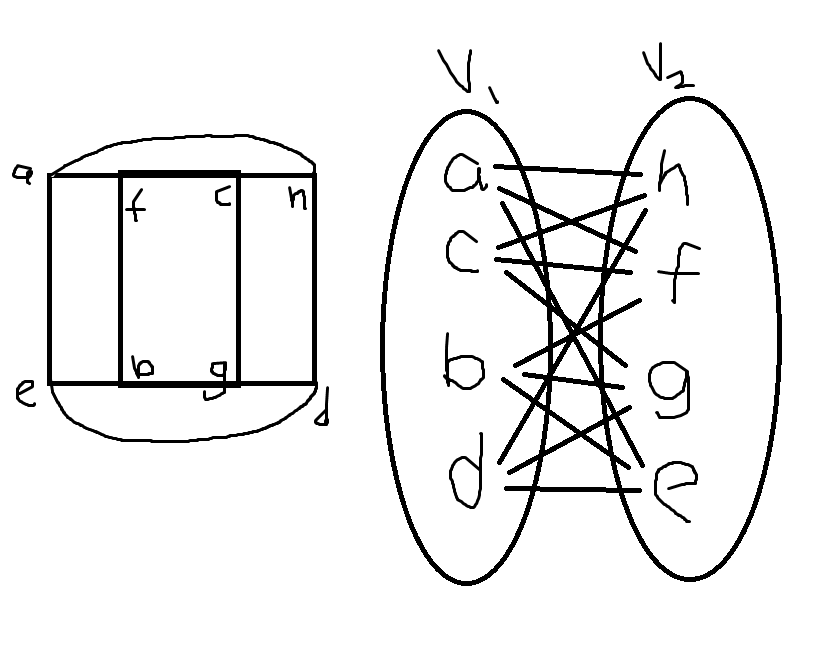
\includegraphics[height=200px]{hw2q16a.png}\newline{}

The second graph is not a bipartite graph.\newline{}
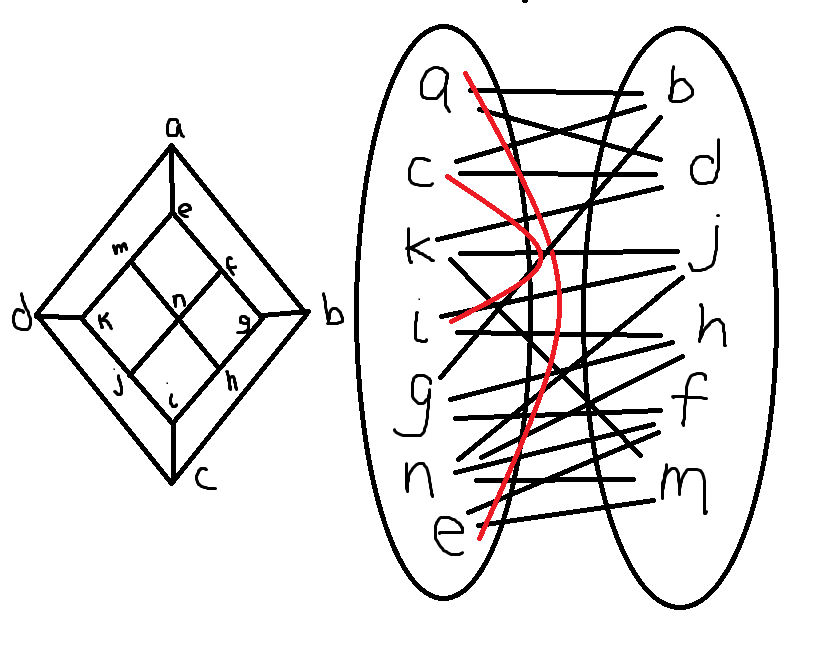
\includegraphics[height=200px]{hw2q16b.png}\newline{}

\end{document}
